\section{Method}

\subsection{Problem Definition}

In UVDT, the vehicle detection and tracking system for single-intersection scenarios adopts a multimodal data fusion architecture.
The input source integrates 3D point cloud data captured by LiDAR and synchronized RGB images from six calibrated cameras, achieving heterogeneous sensor data collaboration through spatiotemporal alignment.
The input for multi-intersection object detection is the same as that for a single intersection, but the input for its object tracking includes trajectories and the corresponding vehicle appearance features. 
The input for the re-identification module is a N×2048 vehicle feature vector. 
The input for the twin part includes trajectory data (comprising the desired vehicle trajectory and the current vehicle state), environmental information (such as road conditions and obstacle information), and the system's control strategy.

\textbf{PointPillars.}
We use the PointPillars network to process the input for vehicle detection and generate the output.
A PointPillars network requires two inputs: pillar indices as a P-by-2 and pillar features as a P-by-N-by-K matrix. P is the number of pillars in the network, N is the number of points per pillar, and K is the feature dimension.
The network begins with a feature encoder, which is a simplified PointNet. It contains a series of convolution, batch-norm, and relu layers followed by a max pooling layer. A scatter layer at the end maps the extracted features into a 2-D space using the pillar indices.
Next, the network has a 2-D CNN backbone that consists of encoder-decoder blocks. Each encoder block consists of convolution, batch-norm, and relu layers to extract features at different spatial resolutions. Each decoder block consists of transpose convolution, batch-norm, and relu layers.
The network then concatenates output features at the end of each decoder block, and passes these features through six detection heads with convolutional and sigmoid layers to predict occupancy, location, size, angle, heading, and class.

\textbf{ReID.}Re-identification is a crucial component of multi-object tracking, aimed at addressing the issue of temporary object occlusion in videos. 
In real-world scenarios, tracked objects may be temporarily obscured by other objects or move out of the camera's field of view, making consistent tracking challenging. 
These objects may also exhibit variations in pose, orientation, and lighting conditions between frames. 
In such complex scenarios, when an object reappears in a new video frame, the tracker often fails to re-identify the object. 
Consequently, the tracker begins to treat the object as a new entity. 
This misidentification leads to errors and inconsistencies in object tracking.

ReID aims to resolve this issue by matching the features of an object in a new frame with those of previously tracked objects, thereby identifying the same object even if it appears in a different location or orientation, or under varying lighting conditions compared to the previous frame. 
This approach ensures that the tracker can maintain consistent tracking information for a given object\cite{Alpher24d}.

\subsection{Single Intersection Multi-Object Tracking}

\textbf{TrackerJPDA.}

\textbf{Single Detection Class Probability Update.}
First, consider the class information association between one detection and one track. 
Assume the confusion matrix of the detection is $C=\left[c_{i j}\right]$, where $c_{i j}$ denotes the likelihood that the classifier outputs the classification as $j$ if the truth class of the target is $i$.
Here, $i,j = 1,…, N$, and $N$ is the total number of possible classes.
At time $k-1$, the probability distribution of a track is given as 
\begin{align}
	\mu(k-1) & = \left[\begin{array}{l}
		\mu_{1}(k-1) \\
		\vdots \\
		\mu_{N}(k-1)
	\end{array}\right]
\end{align}
where $\mu_{i}$ is the probability that the classification of the track is $i$.
If the tracker associates the detection to the track at time $k$, then the updated value of $\mu_{i}$ using Bayes' theorem is
\begin{align}
	\mu_{i}(k) = \frac{c_{i j} \mu_{i}(k-1)}{\sum_{l = 1}^{N} c_{l j} \mu_{i}(k-1)}
\end{align}
Write this equation in a vector form for all possible classifications as
\begin{align}
	\mu(k) & = \frac{c_{j} \otimes \mu(k-1)}{c_{j}^{T} \mu(k-1)}
\end{align}
where $c_{j}$ is the $j$-th column of the confusion matrix and $\otimes$ represents element-wise multiplication. 
This equation represents the updated class probability of a track if the track is associated with the detection of classification $j$.

\textbf{Mixed Association Likelihood in Cluster.}
The tracker performs gating and clustering by using only the kinematic information between detections and tracks. 
After that, in each cluster, the tracker calculates the mixed likelihood of association between a detection $m$ and a track $t$ as:
\begin{align}
	\Lambda(m, t) & = \Lambda_{k}^{1-\alpha}(m, t) \Lambda_{c}^{\alpha}(m, t)
\end{align}
where $\alpha$ represents Weight factor of class likelihood; $\Lambda_{k}$ represents Likelihood of assigning a detection to a track based on the kinematic states; $\Lambda_{c}$ represents Likelihood of assigning a classified detection to a track based on the class information.
In the equation, $\Lambda_{c}$ takes one of these three forms based on the value of $m$ and $t$.

$\bullet$ $m > 0$ and $t > 0$ — A hypothesis that the measurement is associated with a track in the tracker. 
In this case,
\begin{align}
	\Lambda_{k}(m, t) & = c_{j}^{T} \mu(k-1)
\end{align}
where $c_{j}$ is the $j$-th column in the confusion matrix that detection $m$ corresponds to, and $\mu(k-1)$ is the class probability vector of the track in the previous step.

$\bullet$ $m > 0$ and $t = 0$ — A hypothesis that the measurement is not associated with any track in the tracker. In this case,
\begin{align}
	\Lambda_{k}(m, t) & = c_{j}^{T} \mu^{0}
\end{align}
where $c_{j}$ is the $j$-th column in the confusion matrix that detection $m$ corresponds to, and $\mu^{0}$ is the a priori class distribution vector of tracks.

$\bullet$ $m = 0$ and $t > 0$ — A hypothesis that the track is not associated with any measurement in the tracker. In this case,
\begin{align}
	\Lambda_{k}(m, t) & = 1
\end{align}
Using the mixed likelihoods of association between detections and tracks in a cluster, the tracker generates all the feasible events and then calculates the marginal probability of assigning each detection to each track in the cluster.

\textbf{Update Track Class Probability.}
Suppose the marginal probabilities of $M$ detections assigned to a track in the cluster are $\left(\beta_{0}, \beta_{1}, \ldots, \beta_{M}\right)$, where $\beta_{0}$ is the marginal probability that no measurements is associated with the track. 
Then the tracker updates the class probability of the track as
\begin{align}
	\mu_{k} & = \left(\sum_{m = 1}^{M} \beta_{m} \frac{c_{j(m)} \otimes \mu(k-1)}{c_{j(m)}^{T} \mu(k-1)}\right)+\beta_{0} \mu(k-1)
\end{align}
where $c_{j}(m)$ is the class probability vector of detection $m$, $\otimes$ represents element-wise multiplication, $\mu(k-1)$ is the class probability vector of the track in the $k-1$ step, and $\mu(k)$ is the class probability vector of the track in the $k$ step.

The tracker updates the class properties of tracks cluster by cluster.

\textbf{Reference System.}

We placed an imaginary ego-vehicle in the center of the intersection, which serves as a reference system. 
For multi-object tracking we input not only the detection frame, but also the position of the camera and radar relative to the self-vehicle, as well as the position of the ego-vehicle. 
The position coordinates of the self-vehicle in the experiment were always (0,0,0,), i.e. stationary. 
The tracking yielded trajectory coordinates initially relative to the LiDAR, which we also fitted to the world coordinates in Carla.

\textbf{Process}

In this process, we employ a tracker to handle the 2D and 3D bounding boxes obtained from target detection, along with their corresponding timestamps. 
The tracker utilizes a soft assignment strategy, allowing each trajectory to integrate contributions from multiple detection results. 
Its responsibilities include trajectory initialization, confirmation, correction, prediction (including prediction in a coasting state without active motion), and deletion. 
For each trajectory, the tracker estimates its state vector and the covariance matrix of the state estimation error. 
It ensures that every detection is assigned to at least one trajectory; if a detection cannot be matched to any existing trajectory, the tracker creates a new one.

Newly generated trajectories are initially in a tentative state. 
When a tentative trajectory accumulates a sufficient number of detection assignments, its status transitions to confirmed. 
If the detections themselves already carry explicit classification information (i.e., the returned trajectory data contains non-zero fields), the corresponding trajectory is immediately confirmed as valid. 
Once a trajectory is confirmed, the tracker recognizes it as representing a real physical object. 
However, if a trajectory fails to receive any detection assignments within a predefined number of update cycles, it will be deleted.

Through this process, we are ultimately able to obtain the trajectories of vehicles within the intersection.


\subsection{Multi Intersection and Multi-Object Tracking}

In the Town10 scene of the CARLA simulation platform, we configure a differentiated blueprint for each experimental vehicle, so that it strictly follows the preset path from a fixed starting point to a specified end point, and build a fully controllable and highly reproducible dynamic traffic scene.
To achieve all-round data collection, we deploy RGB cameras and semantic segmentation cameras at the front and rear positions of each experimental vehicle, respectively, and use a multi-view synchronous acquisition system to capture the continuous changes in the vehicle's appearance features and spatial posture in real time, and finally generated dynamic ground truth and image sequences with precise spatiotemporal alignment characteristics.

Subsequently, the vehicle images of the front and rear views are cropped based on ground truth and the front and rear view images of the same vehicle are combined to form a dataset of that vehicle, to which the vehicle images of the occluded views are added to form the final dataset.
Finally, the images are reshaped to a size of 224x224.

Finally, the images of vehicles tracked at intersections 1 and 2 are matched with the trained re-identification network.
In other words, the vehicle tracked at the previous intersection is the object that needs to be re-identified, and it will be recognized at the next intersection, allowing the trajectories corresponding to the two vehicles to be integrated.

For matching vehicle trajectories between intersections, we use a re-recognition network to extract features from the vehicle images and then compute the cosine similarity of these two features.
If Intersection 1 has M vehicles and Intersection 2 has N vehicles, a matrix of size M×N is generated. 
If the similarity exceeds a certain threshold, the two vehicles are considered to be the same vehicle.

\textbf{ResNet-50.}
ResNet-50 primarily consists of five main components: an initial convolutional layer, a max-pooling layer, four stages of residual blocks, a global average pooling layer, and a fully connected layer, totaling 50 layers (including convolutional layers, pooling layers, and fully connected layers). 
Among these, the four stages of residual blocks are the core of ResNet-50. 
The number of residual blocks and the size of feature maps for each stage are shown in Table 1.

\begin{table}[t]
	\centering
	\caption{Table of the number of residual blocks and feature map sizes for each stage}
	\label{tab:improved}
	\begin{tabular}{|c|c|c|c|}
		\hline
		\multicolumn{1}{|c|}{Stage} & \multicolumn{1}{c|}{NRB} & \multicolumn{1}{c|}{FMS} & \multicolumn{1}{c|}{NOC} \\
		\hline
		Stage1 & 3 & 56×56 & 256 \\
		\hline
		Stage2 & 4 & 28×28 & 512 \\
		\hline
		Stage3 & 6 & 14×14 & 1024 \\
		\hline
		Stage4 & 3 & 7×7 & 2048 \\
		\hline
	\end{tabular}
\end{table}

The first residual block in each stage performs downsampling on the size of the feature maps, while the subsequent residual blocks maintain the same feature map size.

ResNet-50 employs a residual block structure known as Bottleneck, which aims to reduce computational complexity. 
Each residual block consists of the following layers:

$\bullet$ 1$\times$1 Convolutional Layer: Used for dimensionality reduction, decreasing the number of channels.

$\bullet$ 3$\times$3 Convolutional Layer: Used for extracting spatial features.

$\bullet$ 1$\times$1 Convolutional Layer: Used for dimensionality increase, restoring the number of channels.

$\bullet$ Residual Connection: The input is directly added to the output of the 1x1 convolutional layer. 
If the number of channels or the size of the input and output do not match, a 1x1 convolution is applied to adjust the input.

Each convolutional layer is followed by batch normalization and a ReLU activation function.

\subsection{Trajectory Inference and Reconstruction}

\textbf{Inference of Trajectories in Unknown Regions.}
Upon completing the tracking of all vehicle trajectories, we chronologically sort the trajectory of each vehicle and select the last waypoint of the same vehicle at the previous intersection along with the first waypoint at the next intersection as the starting and ending points of the unknown region. 
These two waypoints are then fed into the navigation algorithm module, which subsequently computes the trajectory between them.

In the Carla simulation environment, vehicle trajectory planning is achieved by utilizing the A* algorithm to search for the shortest path within the graph structure constructed from the topological map. 
The A* algorithm evaluates the comprehensive cost of nodes and, at each step, selects the node with the lowest comprehensive cost for expansion, thereby efficiently guiding the search process towards the target node. 
The core of this algorithm lies in the evaluation function 
\begin{align}
	\mathit{f}(n) & = g(n)+h(n)
\end{align}
where $\mathit{g}(n)$ represents the actual cost from the start node to the current node, and $\mathit{h}(n)$ denotes the estimated cost from the current node to the target node.
During the process of exploring the shortest path using the A* algorithm, if edges with a weight of 0 exist in the graph structure, it may lead to vehicles changing lanes excessively frequently within an extremely short time frame, which contradicts normal driving logic. 
To mitigate this phenomenon, we have introduced a lane-changing penalty mechanism in path planning. 
Specifically, for nodes involving different lanes, we have added a penalty term, ensuring that the distance calculation between nodes is not only based on spatial distance but also takes into account the frequency of lane changes. 
Originally, $\mathit{h}(n)$ was calculated by directly measuring the distance between nodes, which is represented as
\begin{align}
	\mathit{h}(n) & = d\left(w p_{1}, w p_{2}\right)
\end{align}
where $w p_{1}, w p_{2}$ denote the nodes and $d$ denotes the Euclidean distance. 
And in our navigation algorithm,
\begin{align}
	\mathit{h}(n) & = d\left(w p_{1}, w p_{2}\right)+\lambda \cdot\left|l_{1}-l_{2}\right|
\end{align}
where $\lambda$ denotes the weights and $l_{1}, l_{2}$ denotes the lanes.


\textbf{All Trajectory Restoration.}
Through the aforementioned algorithmic framework, we are able to obtain vehicle trajectories in unknown regions. 
Simultaneously, we have also acquired vehicle trajectories at intersections using the JPDA tracker. 
At this point, we only need to concatenate all trajectories of the same vehicle in chronological order and place them into a new collection, thereby obtaining the complete trajectory of that vehicle. 
This method can be represented as: 
\begin{align}
	S(t) = \bigcup_{i=1}^{N} \Bigl( T_i(t) \cup f\Bigl( \lim_{\!t \to t_i^+} T_i(t), \lim_{\!t \to t_{i+1}^-} T_{i+1}(t) \Bigr) \Bigr)
\end{align}
where $S$ is the trajectory collection, $T_i(t)$ represents the previous trajectory. 
The limits $\lim_{t \to t_i^+} T_i(t)$ and $\lim_{t \to t_{i+1}^+} T_{i+1}(t)$ correspond to the end waypoint of the $i$-th trajectory and the start waypoint of the $(i+1)$-th trajectory, respectively.
As demonstrated in Fig. \ref{fig:3}, we can derive the complete vehicle trajectory collection, effectively reconstructing the trajectories of all vehicles.
\begin{figure}[t]
	\centering
	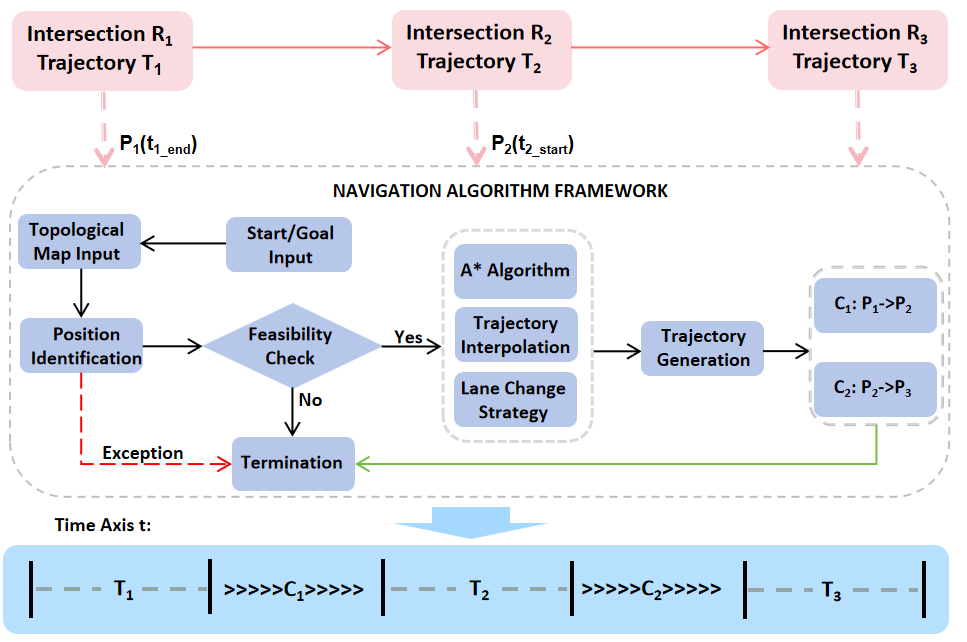
\includegraphics[width=\linewidth]{picture/picture3.png} 
	\caption{Trajectory restoration schematic} 
	\label{fig:3} 
\end{figure}

\subsection{Twin of Trajectory}

Through the previous steps, we have obtained the trajectories of all vehicles. 
Here, we will further optimize these trajectories using a trajectory smoothing algorithm, and then employ a PID controller to control the vehicles, ensuring they follow the optimized trajectories\cite{Alpher22d}. 
The PID controller consists of three main components: Proportional control (P), Integral control (I), and Derivative control (D). Each component serves a specific purpose, enabling the regulation of different aspects of the system.

$\bullet$ The proportional control component adjusts the control output directly based on the current error. 
The control output is proportional to the error, meaning that the larger the error, the stronger the control action. 
The formula is as follows:
\begin{align}
	u_{P}(t) & = K_{p} \cdot e(t)
\end{align}
Here, $K_{p}$ is the proportional gain, which determines the strength of the proportional control's response to the error.

Proportional control can quickly respond to errors and reduce their magnitude.
However, using only proportional control may not completely eliminate steady-state error, which is the small error that remains after the system has stabilized.

$\bullet$ The integral control component accumulates the sum of errors and adjusts the control output based on this accumulated value. 
The integral term takes into account historical errors and is capable of eliminating steady-state errors. 
The formula is as follows:
\begin{align}
	u_{I}(t) & = K_{i} \int_{0}^{t} e(\tau) d \tau
\end{align}
Here, $K_{i}$ is the integral gain, which determines the strength of the integral control's response to the accumulated error. 

By considering the accumulated error, integral control can eliminate steady-state errors, enabling the system to achieve the target value over the long term. 
However, excessively high integral gain may lead to system overshoot or oscillation.

$\bullet$ The derivative control component adjusts the control output based on the rate of change of the error. 
It predicts future error trends and takes preemptive measures. 
The formula is as follows:
\begin{align}
	u_{\mathit{D}}(t) & = K_{d} \cdot \frac{d e(t)}{d t}
\end{align}
Here, $K_{d}$ is the derivative gain, which determines the strength of the derivative control's response to the rate of change of the error.

Derivative control can suppress rapid changes in errors, reduce system overshoot and oscillation, and make the system response smoother. 
However, derivative control is sensitive to noise and can amplify high-frequency noise.


The tuning process of the PID controller is as follows:  
1. Calculate the error $e(t)$ between the target value (setpoint) and the current system output in real time.  
2. Compute the proportional action $K_{p} \cdot e(t)$ based on the current error, the integral action $K_{i} \int_{0}^{t} e(\tau) d \tau$ based on historical errors, and the derivative action $K_{d} \cdot \frac{d e(t)}{d t}$ based on the rate of change of the error.  
3. Sum the results of the proportional, integral, and derivative components to obtain the final control output $u(t)$, which is then applied to the system (for example, adjusting the vehicle's acceleration or direction). 
4. The system adjusts based on the control output $u(t)$, changing its state (for example, speed, position, etc.). 
The controller continues to monitor the system state, updates the error in real time, and repeats the above steps until the system stabilizes near the target value.


\subsection{Evaluation}

We employed two evaluation metrics.

\textbf{Multiple Object Tracking Accuracy.}
Single-camera, multi-object tracking performance is typically measured by the Multiple Object Tracking Accuracy (MOTA):
\begin{align}
	\mathit{MOTA} & = 1-\frac{F N+F P+M}{T}
\end{align}
Among them:
$FN$ (False Negatives) represents the number of missed detections, which means targets that truly exist but were not detected.
$FP$ (False Positives) represents the number of false detections, which means targets that were detected but do not actually exist.
$M$ (Mismatches) represents the number of identity mismatches, which means cases where the tracking ID of a target was incorrectly assigned during the tracking process.
$T$ (Total number of true detections) represents the total number of true detections, which means the number of targets correctly detected across all frames.

The value of MOTA ranges from 0 to 1, with higher values indicating better tracking performance. 
A MOTA of 1 means there are no missed detections, false detections, or identity mismatches, representing perfect tracking performance. 
A MOTA of 0 means the tracking performance is very poor, with all detections being incorrect.

\textbf{Multi Camera Tracking Accuracy.}
The multi-camera object tracking accuracy (MCTA) which condenses all aspects of system performance into one measure\cite{Alpher23b}:
\begin{align}
	\mathit{MCTA} & = \frac{2 P R}{P+R}\left(1-\frac{M^{w}}{T^{w}}\right)\left(1-\frac{M^{h}}{T^{h}}\right)
\end{align}
Among them:
$P$ represents the proportion of correct matches (correctly identifying and tracking targets) across all cameras.  
$R$ represents the recall rate, which is the proportion of all true targets that are correctly tracked.  
$M^{w}$ represents the number of weak matching errors, which is the number of times a target is incorrectly matched to another target during the tracking process.  
$T^{w}$ represents the total number of weak matching attempts, which is the total number of possible matching attempts.  
$M^{h}$ represents the number of strong matching errors, which is the number of times a target is incorrectly matched to another target during the tracking process, but here it may refer to a stricter standard for matching errors.  
$T^{h}$ represents the total number of strong matching attempts, which is the total number of possible matching attempts.

MCTA evaluates tracking accuracy by considering the proportion of correct matches and the recall rate, while also assessing tracking consistency by penalizing weak and strong matching errors. 
The higher the MCTA value, the better the performance of the multi-camera tracking system.
